
%version 2: \usepackage{hyperref}


%%%%%%%%%%%%%%%%%%%%%%%%%%%%%%%%%%%%%%%%%%%%%%%%%%%%%%%%%%%%%%%%%%%%%%%%
%Para las ecuaciones siempre es Ec.(n).
%Para las figuras siempre es Fig.n, incluso en el caption de la figura. Tambien las Tablas
%Para las referencias es [n]
%%%%%%%%%%%%%%%%%%%%%%%%%%%%%%%%%%%%%%%%%%%%%%%%%%%%%%%%%%%%%%%%%%%%%%%%

\documentclass[
reprint,
%notitlepage,
%superscriptaddress,
%groupedaddress,
%unsortedaddress,
%runinaddress,
%frontmatterverbose, 
%preprint,
%showpacs,preprintnumbers,
%nofootinbib,
%nobibnotes,
%bibnotes,
%11 pt,
amsmath,
amssymb,
%aps,
%pra,
prb,
%rmp,
%tightenlines %esto hizo el milagro de sacar los espacios en blancos estocásticos (?)
%prstab,
%prstper,
%floatfix,\textbf{}
]{revtex4-1} %Instalar primero para usarlo. Paquete malo.

%\documentclass[onecolumn, aps, amsmath,amssymb ]{article}
\usepackage{lipsum}  
\usepackage{graphicx}% Include figure files
\usepackage{subfig}
\usepackage{braket}
\usepackage{comment} %comment large chunks of text
\usepackage{dcolumn}% Align table columns on decimal point
\usepackage{bm}% bold math
%\usepackage{hyperref}% add hypertext capabilities
\usepackage[mathlines]{lineno}% Enable numbering of text and display math
%\linenumbers\relax % Commence numbering lines
\usepackage{mathtools} %% Para el supraíndice

\usepackage[nice]{nicefrac}

%%%%%%%El Señor Español%%%%%%%%%%%%%%%%%%%%%%%%%%%
\usepackage[utf8]{inputenc} %acento
\usepackage[
spanish, %El lenguaje.
es-tabla, %La tabla y no cuadro.
activeacute, %El acento.
es-nodecimaldot %Punto y no coma con separador de números
]{babel}
\usepackage{microtype} %para hacerlo más bonito :33 como vos (?) 
%%%%%%%%%%%%%%%%%%%%%%%%%%%%%%%%%%%%%%%%%%%%%%%%%%%
%%%%%%%%% Para que las imágenes se queden dónde las quiero (?
\usepackage{float}
%%%%%%%%%%
\usepackage{enumitem}
\usepackage{hyperref} % Para usar \url

%%%%%%%%Cambia a Fig de Figure%%%%%%%%%%
\makeatletter
\renewcommand{\fnum@figure}{Fig. \thefigure} 
\makeatother
%%%%%%%%%%%%%%%%%%%%%%%%%%%%%%%%%%%%%%%%
\raggedbottom

\usepackage{multirow}
\begin{document}

\title{Práctica 6: Método basado en Árboles de Decisión}
\author{Evelyn G. Coronel}

\affiliation{Redes Neuronales y Aprendizaje Profundo para Visión Artificial\\ Instituto Balseiro\\}

\date[]{\lowercase{\today}} 

\maketitle

\section*{Ejercicio 1}

% (a)  Separar los datos en dos particiones, una para datos de entrenamiento/validación (osea, de desarrollo) y otra para test.

\subsection*{Item A}
Este ejercicio, se utilizan arboles de clasificación y regresión para obtener la cantidad de unidades de asientos para bebés se compran, en función de las características del producto y del lugar donde se venden. Las variables a tener en cuenta del conjunto de datos son:

\begin{enumerate}
    \item Sales: Cantidad de asientos vendidos en una tienda.
    \item CompPrice: Precio del asiento según la competencia.
    \item Income: Ingreso de dinero medio en miles de USD del lugar donde se localiza la tienda.
    \item Advertising: Inversión en propaganda de la tienda en  miles de USD.
    \item Population: Población local en miles.
    \item Price: Precio de venta por cada asiento.at each site
    \item ShelveLoc: Posición del asiento en las góndolas, se clasifica las posición como Bad, Good and Medium  (Malo, Bueno y Medio).
    \item Age: Edad promedio de la población local.
    \item Education: Nivel de educación
    \item Urban: \emph{Yes} si la tienda está ubicada en un lugar urbano, \emph{No} caso contrario.
    \item US:\emph{Yes} si la tienda está ubicada en Estados Unidos, \emph{No} caso contrario.    
\end{enumerate}
Además de estas variables, se agregó una última variable llamada \emph{High} es \emph{Yes} si las ventas superan las $8$ unidades, \emph{No} caso contrario. 

Para realizar los ajustes, se transformaron los datos descriptos \emph{Yes} y \emph{No} como 1 y 0 respectivamente, y \emph{Good}, \emph{Medium}, \emph{Bad} con 3, 2 y 1. Además se separó el conjunto de datos en un $80\%$ de entrenamiento y un $20\%$ de validación. Las variables \emph{Sales} y \emph{High} se separan del resto de los atributos para hacer los ajustes.

% (b)  Entrenar un árbol de decisión para clasificación de la variableHigh. Hacer un plot delárbol (usarscikit-learn) e interpretar los resultados.
\subsection*{Item B}

Usando un árbol de decisión de clasificación, se utilizó la columna \emph{High} como salida esperada y el resto de los atributos como entrada. El árbol está instanciado de tal forma que  el ajuste se realice hasta que las hojas sean puras, es decir, que el coeficiente de gini del nodo sea 0. Con esto se obtuvo un árbol con las  características que se presentan en la Tabla~\ref{tab:item_B}. 

\begin{table}[H]
    \begin{small}
        \begin{center}
            \begin{tabular}[c]{l|l}
                Profundidad & 11 \\
                Hojas & 50 \\
                Error de entrenamiento & 0 de 320\\
                Precisión de entrenamiento & 1 \\
                Error de validación & 3 de 80\\
                Precisión de validación & 0.6625 \\
            \end{tabular}
        \end{center}
    \end{small}
    \caption{Características del árbol de decisión de clasificación posterior al ajuste}
    \label{tab:item_B}
\end{table}

Las primeras dos ramas del árbol se muestran en la Fig.\ref{fig:item_B_tree}. En este caso se llega hasta un profundidad de 11 porque no estamos limitando el valor de gini de las hojas, la clasificación  se realiza hasta que los datos de entrenamiento tengan una clasificación fiel, por eso se observa el overfitting del árbol. El primer nodo usa la posición en la góndola   para clasificar los datos, ya que este parámetro divide mejor los datos, dicho de otra forma, tiene el coeficiente de gini mayor de todos los nodos.

\begin{figure}[H]
    \begin{small}
        \begin{center}
            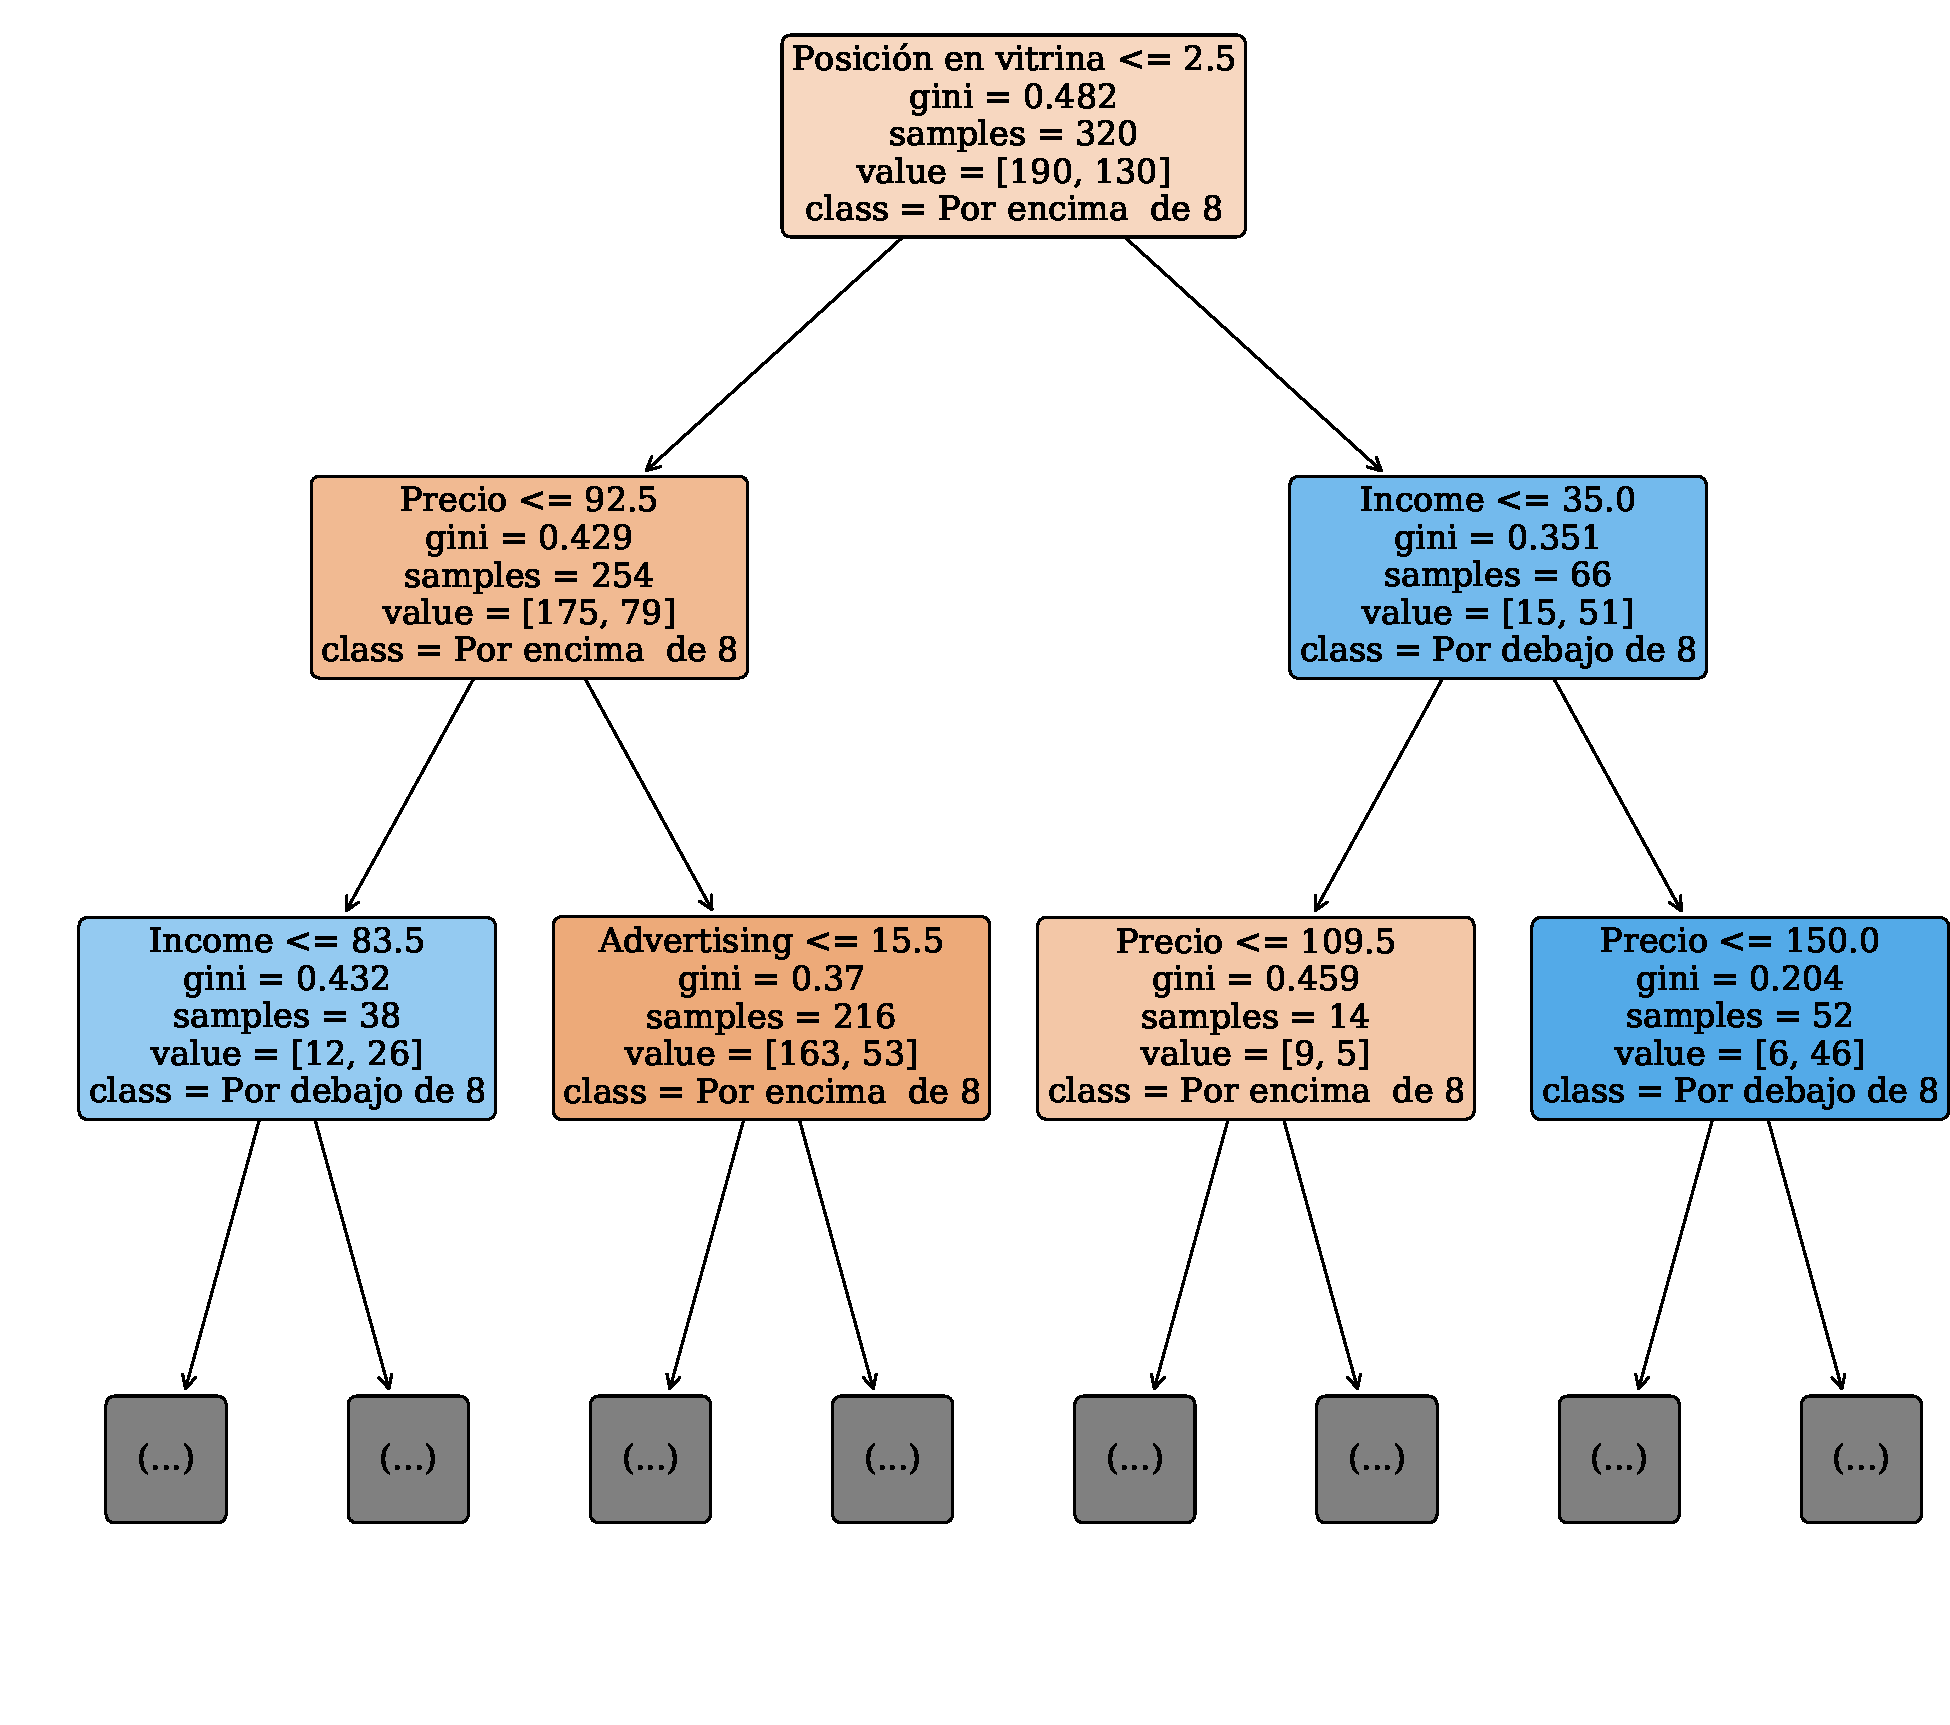
\includegraphics[width=0.5\textwidth]{figures/tree_B_tree.pdf}
        \end{center}
        \caption{Las primeras dos ramas de la estructura del árbol de clasificación para el item B.}
        \label{fig:item_B_tree}
    \end{small}
\end{figure}


% (c)  Entrenar un árbol de decisión para regresión de la variableSales.  Hacer un plot delárbol (usarscikit-learn) e interpretar los resultados.
\subsection*{Item C}

El árbol instanciado en este item es el árbol de regresión, los parámetros por defecto también hacen que el árbol regresione hasta tener hojas con gini nulo. Como se ven en la Tabla \ref{tab:item_C} se muestran las características del árbol luego de realizar el ajuste. Nuevamente se tiene un overfitting con el conjunto de entrenamiento. 

Tal como el caso del árbol de clasificación, el atributo que mejor separa los datos es la posición de los asientos en las góndolas. Esto tiene sentido porque eso es independiente del tipo de árbol que se utilize.

\begin{table}[H]
    \begin{small}
        \begin{center}
            \begin{tabular}[c]{l|l}
                Profundidad & 18 \\
                Hojas & 320 \\
                Error de entrenamiento & 0.0\\
                Precisión de entrenamiento & 1 \\
                Error de validación & 0.07\\
                Precisión de validación & 0.2759 \\
            \end{tabular}
        \end{center}
    \end{small}
    \caption{Características del árbol de regresión posterior al ajuste}
    \label{tab:item_C}
\end{table}

\begin{figure}[H]
    \begin{small}
        \begin{center}
            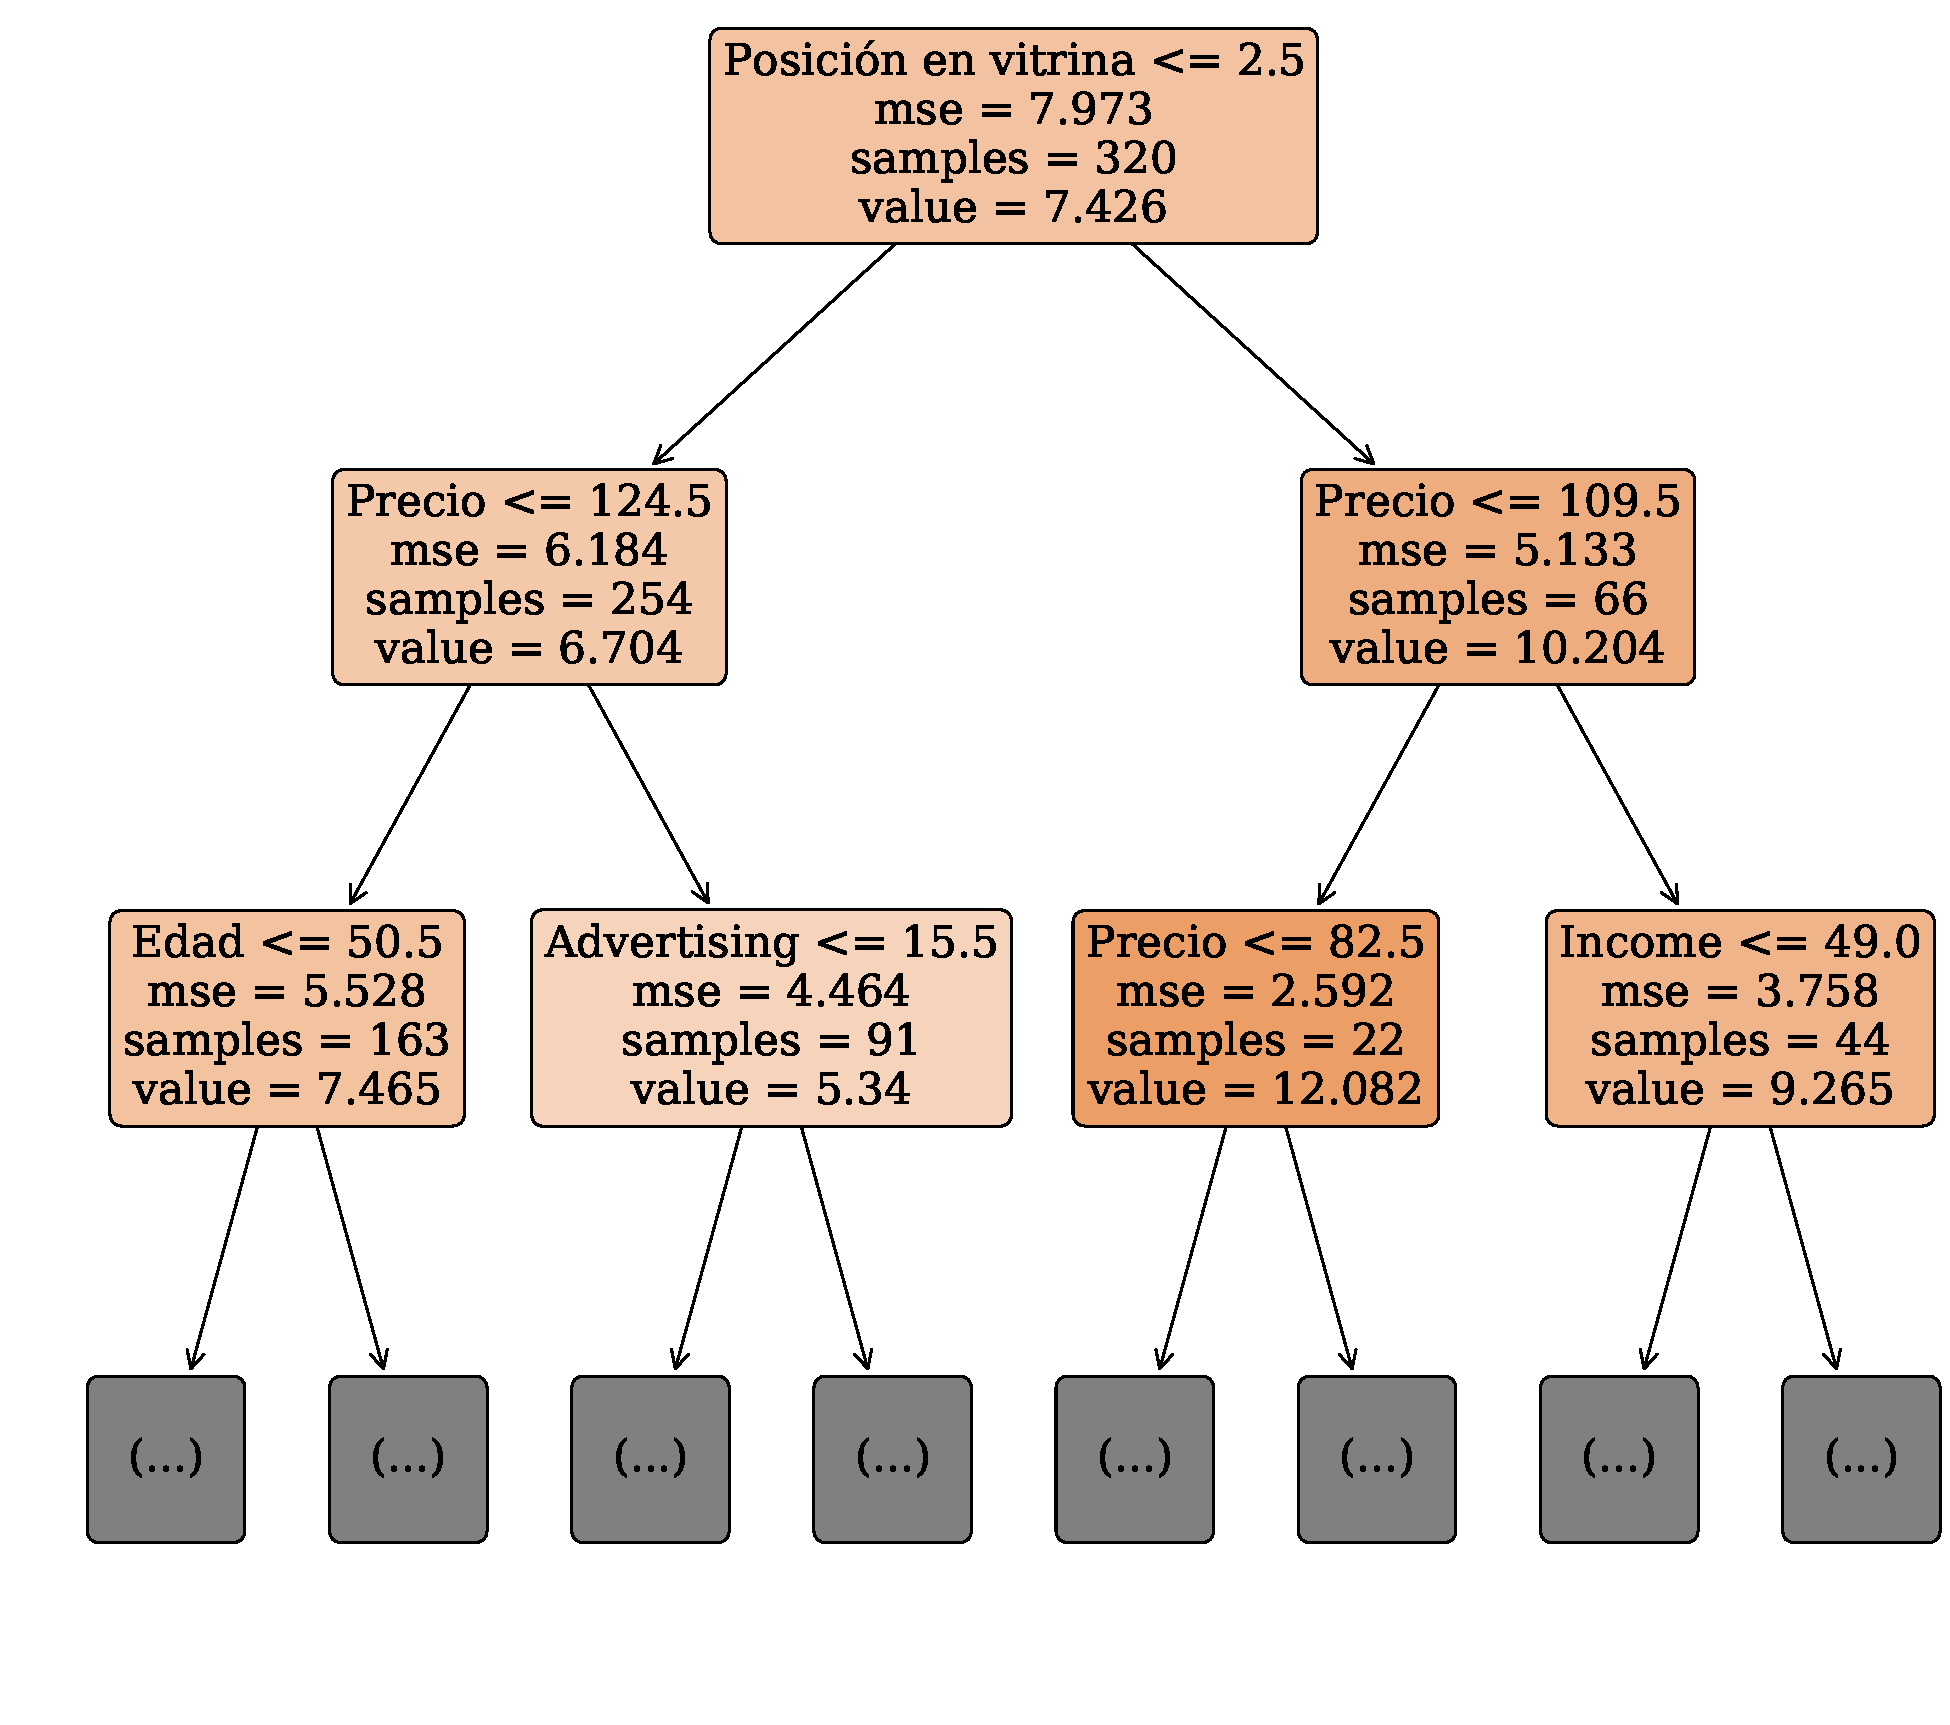
\includegraphics[width=0.5\textwidth]{figures/tree_C_tree.pdf}
        \end{center}
        \caption{Las primeras dos ramas de la estructura del árbol de clasificación para el item C.}
        \label{fig:item_C_tree}
    \end{small}
\end{figure}

A pesar del overfitting del árbol, el árbol aprende la correlación de los atributos con la cantidad de asientos. Esto se observa en la Fig.\ref{fig:item_C_scatter}, dado que los ejes x e y son la cantidad de asientos reales y predichos, mientras más cerca estén los puntos a la línea, mejor es la predicción del árbol.
\begin{figure}[H]
    \begin{small}
        \begin{center}
            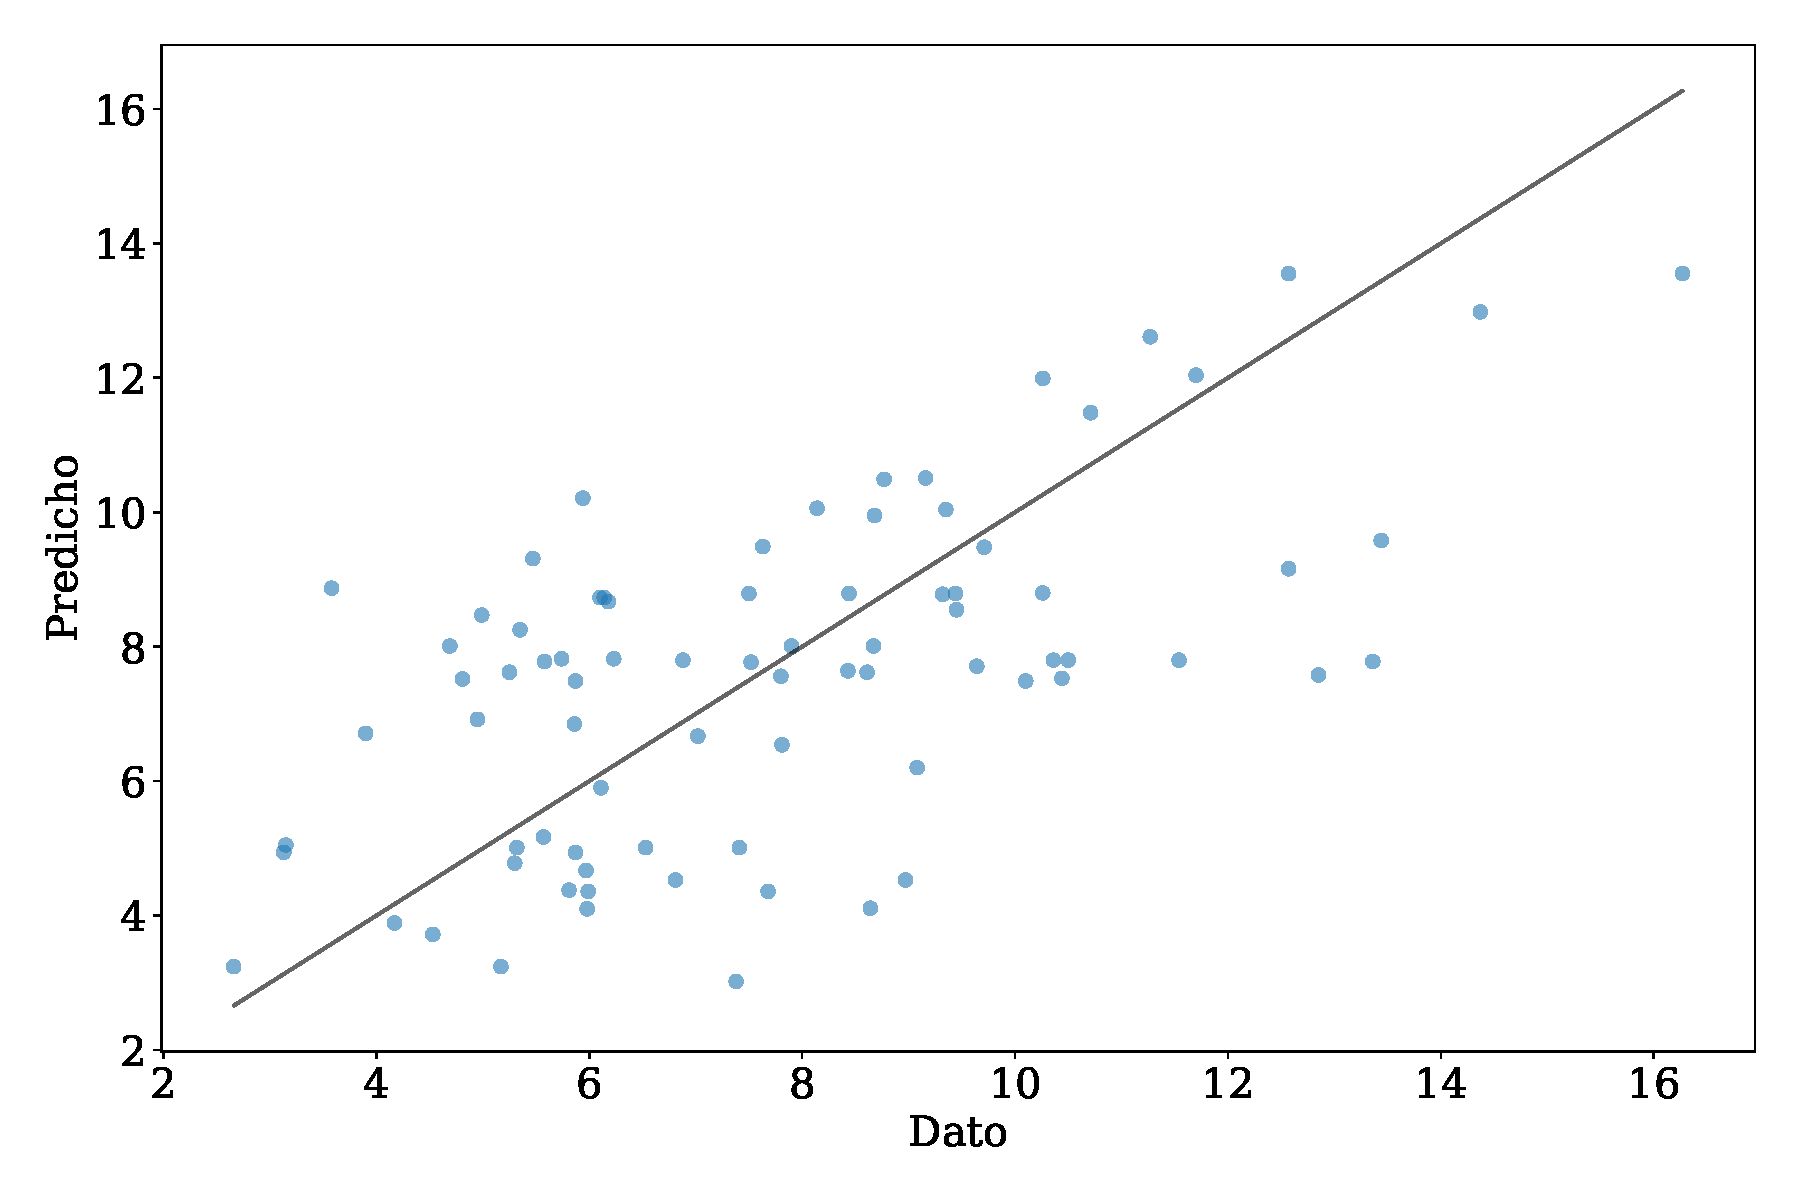
\includegraphics[width=0.5\textwidth]{figures/fit_C_tree.pdf}
        \end{center}
        \caption{Comparación entre el dato y la predicción del árbol de regresión para else item C.}
        \label{fig:item_C_scatter}
    \end{small}
\end{figure}

% (d)  ¿Cuál es el error de test que obtienen en cada caso?  Comparar con el error de entrenamiento y determinar si tienen overfitting o no.
\subsection*{Item D}


% (e)  Para el árbol de regresión, usarcross-validationpara determinar el nivel óptimo de com-plejidad del árbol.  Busquen cómo usar enscikit-learnla técnica depruningparamejorar la tasa de error de test.
\subsection*{Item E}


% (f)  Para el caso de regresión,  usar el abordaje tipobaggingpara mejorar el error de test.Comparar con el abordaje de un único árbol de decisión.  Buscar enscikit-learncómo determinar el orden de importancia de los atributos.
\subsection*{Item F}

% (g)  Usarrandom forestspara mejorar los resultados datos. Comparar el error de test con losabordajes anteriores.  ¿Cambia el orden de la importancia de los atributos?  Hacer unplot con el error de test en función del del hiperparámetromax_featuresque limitael número de atributos a incluir en cada split.  Hacer otro plot equivalente en funcióndemax_depth.1
\subsection*{Item G}

% (h)  Hacer la misma regresión usandoAdaBoosty comparar errores de test con lo obtenidoconRandom Foresten el punto anterior.2
\subsection*{Item H}

\end{document}